\section{Software Switches \glsentryshort{sdn}}
\label{sec:softSwitchs}

En las redes definidas por software, los software switches desempeñan un papel fundamental al permitir la virtualización y la gestión centralizada de las redes. Estos switches, a diferencia de los switches de hardware tradicionales, se implementan como software y se ejecutan en servidores convencionales. Un software switch en \gls{sdn}, en adelante \textit{softswitch}, es una entidad lógica que reside generalmente en una instancia virtual o en un servidor, y se comunica con el controlador \gls{sdn} para recibir instrucciones sobre cómo procesar los paquetes de datos que fluyen a través de la red. Al estar basados en software, estos switches pueden ser escalados y desplegados de manera flexible según las necesidades y demandas de la red. La principal ventaja de los \textit{softswitches} radica en su capacidad para adaptarse y responder de manera dinámica a las necesidades de la red. Pueden implementar diferentes funciones de red, como enrutamiento, conmutación, balanceo de carga y seguridad, a través de la instalación de reglas desde el controlador \gls{sdn}. \\
\\
% fig
\begin{figure}[ht]
    \centering
    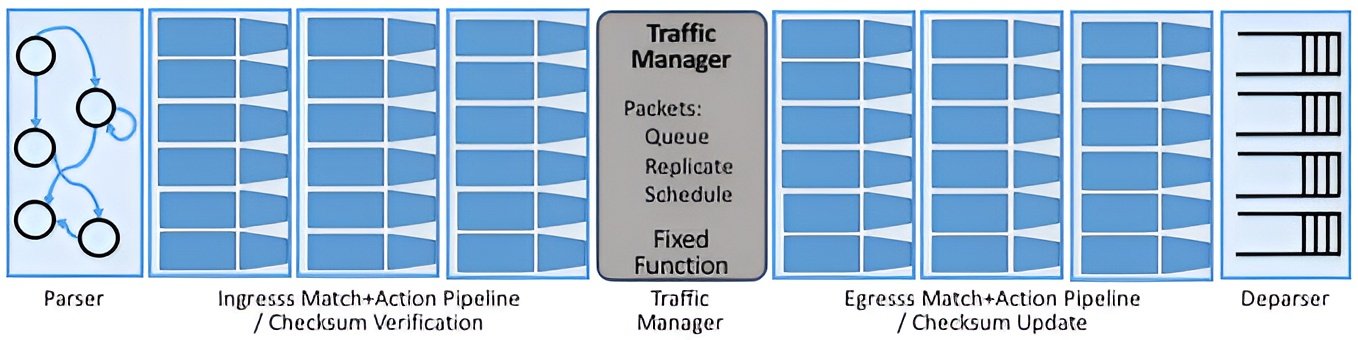
\includegraphics[width=0.8\textwidth]{archivos/img/teoria/softswitch.jpg}
    \caption{Arquitectura genérica de un \textit{softswitch} \gls{sdn} \cite{softswitches1}}
    \label{fig:softswitch}
\end{figure}

Según se puede apreciar en la figura \ref*{fig:softswitch}, la arquitectura genérica de un \textit{softswitch} se puede resumir en los siguientes bloques. El primero de todos tiene que ser un parser, que vaya inspeccionando los paquetes entrantes a la pipeline de procesamiento del switch para identificar que tipo es. Una vez se ha identificado el paquete que se va a procesar, el siguiente bloque son las tablas de \textit{match-action}, las cuales tienen una interfaz de comunicación con el controlador \gls{sdn} para establecer criterios y campos de \textit{match}, y en caso de haber un \textit{match}, definir una serie de acciones para llevar a cabo. En función del \textit{softswitch}, la verificación de \textit{checksum}\footnote{Suma de comprobación, campo para comprobar la integridad del paquete de datos} se puede llevar a cabo en el parser o en la etapa de las tablas de \textit{match-action}. El siguiente bloque que nos podemos encontrar en un \textit{softswitch} es el conocido como gestor de tráfico, que variará en función de la implementación, pero nos proveerá de gestión de colas, \gls{qos}, duplicado de paquetes, etc. La siguiente etapa ya es más opcional, que se suele denominar como \textit{egress match-action}, la cual se puede utilizar para definir algún tipo de lógica a la salida de los switches, aunque en la realidad se suele utilizar para actualizar los campos  de \texttt{TTL} y recalcular el \textit{checksum} dado que el paquete se habrá visto modificado. El último bloque es el deparser, el cual se encarga de ensamblar de nuevo el paquete y prepararlo para sacarlo por el puerto de salida del switch.

\subsection{OVS}
\label{subsec:OVS}

OVS (Open vSwitch) es un software switch de código abierto diseñado específicamente para su uso en redes definidas por software (SDN). Es uno de los software switches más utilizados y ampliamente adoptados en entornos SDN debido a su flexibilidad y funcionalidades avanzadas.

Open vSwitch actúa como un switch virtual, proporcionando capacidades de conmutación y enrutamiento para máquinas virtuales y contenedores en entornos de virtualización. Puede ejecutarse en hipervisores populares, como KVM (Kernel-based Virtual Machine), Xen y VMware, y también puede ser implementado como un switch independiente en sistemas operativos de servidor.

Las características clave de Open vSwitch incluyen:

1. Controlador SDN: Open vSwitch se puede controlar y programar mediante un controlador SDN, como OpenDaylight o ONOS. Esto permite una gestión centralizada y un control más granular de la red, así como la implementación de políticas de red definidas por software.

2. Funcionalidades avanzadas: OVS ofrece una amplia gama de funcionalidades, como enrutamiento, balanceo de carga, aislamiento de red, seguridad y calidad de servicio (QoS). Estas características permiten una gestión eficiente de la red y la implementación de políticas específicas para satisfacer las necesidades de las aplicaciones y usuarios.

3. Segmentación de red: Open vSwitch es compatible con la segmentación de red, lo que permite la creación de redes virtuales (network slices) dentro de una infraestructura compartida. Esto permite el aislamiento y la asignación de recursos personalizados para diferentes aplicaciones o usuarios, mejorando la seguridad y el rendimiento de la red.

4. Integración con tecnologías de virtualización: OVS se integra estrechamente con tecnologías de virtualización como OpenStack y Docker. Puede proporcionar conectividad de red entre máquinas virtuales, contenedores y hosts físicos, facilitando la migración y la gestión de recursos en entornos virtualizados.

5. Extensibilidad y soporte para estándares: Open vSwitch es altamente extensible y se puede ampliar mediante la integración de módulos y complementos personalizados. Además, cumple con los estándares de la industria, como el protocolo OpenFlow, para garantizar la interoperabilidad con otros componentes SDN.

En resumen, Open vSwitch (OVS) es un software switch SDN ampliamente utilizado que proporciona capacidades avanzadas de conmutación y enrutamiento para entornos de virtualización. Su flexibilidad, funcionalidades avanzadas, segmentación de red y compatibilidad con estándares lo convierten en una opción popular para implementaciones SDN en diversos entornos, desde centros de datos hasta infraestructuras de proveedores de servicios.

\subsection{BOFUSS}
\label{subsec:BOFUSS}